\documentclass[11pt,a4paper]{article}

\newcommand{\ROOT}[0]{/Users/atlytle/Dropbox/Tex_docs}
\usepackage{\ROOT/jheppub}
\usepackage{\ROOT/mystyle}
\graphicspath{{./figs/}}

\newcommand{\Dmix}[0]{\Delta_{\text{mix}}}

\title{\boldmath $\Delta_\text{mix}$ for overlap on a HISQ sea.}
\author{S.\ Basak,}
\author{A.T.\ Lytle,}
\author{N. Mathur,}
\author{...}
\abstract{...}

\begin{document}
\maketitle
\section{Research}
We have in mind something along the lines of~\cite{Lujan:2012wg} which looks at overlap
on domain-wall.  The ``master formula'' involves pseudoscalar meson masses determined
using propagators calculated from both valence and sea Dirac operators.
A similar approach is used in~\cite{Aubin:2008wk} for domain-wall on asqtad.
The determination of $a^2 \Dmix$ extends the work of~\cite{Orginos:2007tw} to the fine asqtad ensemble.
The prior work computed on only the coarse and uses yet another parametrization which 
appears well-justified based on that paper's discussion.
For overlap on HISQ the pseudoscalar
masses at LO are given as:
\begin{align}
m^2_{vv'} &= B_{\text{ov}} (m_v + m_{v'}) \label{vv'} \\
m^2_{ss'} &= B_{\text{HISQ}}(m_s + m_{s'}) + a^2 \Delta_{t} \label{ss'}\\
m^2_{vs} &= B_{\text{ov}} m_v + B_{\text{HISQ}} m_s + a^2 \Dmix \label{vs}
\end{align}
$\Delta_t$ measures taste-breaking and in particular vanishes for the taste-5 GB pion.
I am unclear on whether there is an additional $\Delta_{\text{sea}}$ term
arising in~\eqref{ss'} and~\eqref{vs} when the valence sea-mass doesn't match the sea mass,
but it looks like there is not such a term.. I need to understand this better.
Some theory references:~\cite{Aubin:2003mg,Bar:2005tu,Chen:2006wf}.
\subsection{Theoretical Background \& Motivation.}
At LO in the chiral expansion, the mixed-action Lagrangian has only one additional low-energy 
constant $C_\text{mix}$~\cite{Bar:2005tu}.  
\be
\mathcal{L_{\text{LO}}} \ni -C_{\text{mix}} \langle \tau_3 \Sigma \tau_3 \Sigma^\dagger \rangle
\ee
This enters into the tree-level expression~\eqref{vs} as
$\Dmix = 16 \,C_\text{mix}/{f^2}$.

A discussion with Nilmani and Saumen generated some interesting questions.
One of these was why we might want $\Dmix$, when we are interested in valence quantities
like \eqref{vv'}.
In general, mixed pions composed of one valence quark and one sea quark will run in loops.  
$\Dmix$ will show up in these propagators.
There are quantities where $\Dmix$ is absent through NLO 
(the valence pion in our case is one such example~\cite{Chen:2006wf,Bar:2003mh}), 
but this is not always the case. (For a general discussion of how $\Dmix$
can affect chiral formulae, see~\cite{Chen:2007ug}).
As two examples where $\Dmix$ affects NLO, we have the nucleon mass~\cite{Tiburzi:2005is} 
(see e.g.\ Eq.(33) of~\cite{WalkerLoud:2008bp} terms involving $\tilde{m}_{ju}$),
and $f_\pi$~\cite{Bar:2005tu,Chen:2006wf}.

A second question was how will knowledge of $\Dmix$ be used in the chiral extrapolations.
One thing that seems clear is that these are not simple $a^2$ effects that can be fit away via the continuum extrapolation.  
\cite{WalkerLoud:2008bp} seems like a good place to start for better understanding this.

\subsection{``Wilsonized'' staggered propagators.}
Ref.~\cite{Orginos:2007tw} has details of constructing the ``Wilsonized" propagator
from the staggered propagator, i.\ e.\ a 4-component object,
and also many useful details regarding the fit-forms of the two-pt functions.  I think is just the inverse
of the Wilson $\rightarrow$ staggered transformation, and it is implemented in {\tt inline\_stag\_to\_wils.cc} in Chroma.


%---- Overlap propagators. ----
\subsection{Overlap on HISQ propagators}
\subsubsection{Measurement Strategy}
I am successfully parsing the overlap propagators, with results for pion correlators that agree
with Nilmani for both single and double mass propagators.  We need to discuss what all data is available and where (including what I may have already), and how much of that we want to run the measurements on..

For the time being I have chosen masses 
0.001000, 0.002000, 0.006000, 0.009000, 0.016500, 0.024000, 0.038000, 0.073100, 0.525000.
These provide a good range and had the most available configurations on {\tt wilson}.
These I have transferred to {\tt overlap/} directory of {\tt brood}.
Ajay collected additional propagators from various directories on BG/P, and I have symlinked
those with the appropriate masses into {\tt overlap/}.

\subsubsection{Results}


%---- HISQ propagators. ----
\subsection{HISQ propagators.}
Right now we are looking at the $24^3 \times 64$ HISQ ensembles with dynamical charm~\cite{Bazavov:2012xda}.
We have unitary propagators for the following masses (cf  Table IX p.16):
\begin{verbatim}
6.00(24^3X64) : 0.0102(m_l) 0.0509(m_s) 0.635(m_c)
6.30(32^3X96) : 0.0074 (m_l) 0.037(m_s) 0.440
6.72(48^3X144) : 0.0048 (m_l) 0.024(m_s) 0.286
\end{verbatim}
On $24^3 \times 64$ there are 81 configurations.

I find that the ``kaon'' effective mass plots have an oscillatory behavior, as compared to 
the pions.  
%For example see Fig.[].  
I would like to understand this better.
In practice I still fit the standard cosh form because I think the oscillating state has a much higher mass. Preliminary results for all combination of HISQ masses are in Fig.~\ref{HH_pseudo}.% and [].
\begin{figure}[h]
\centering
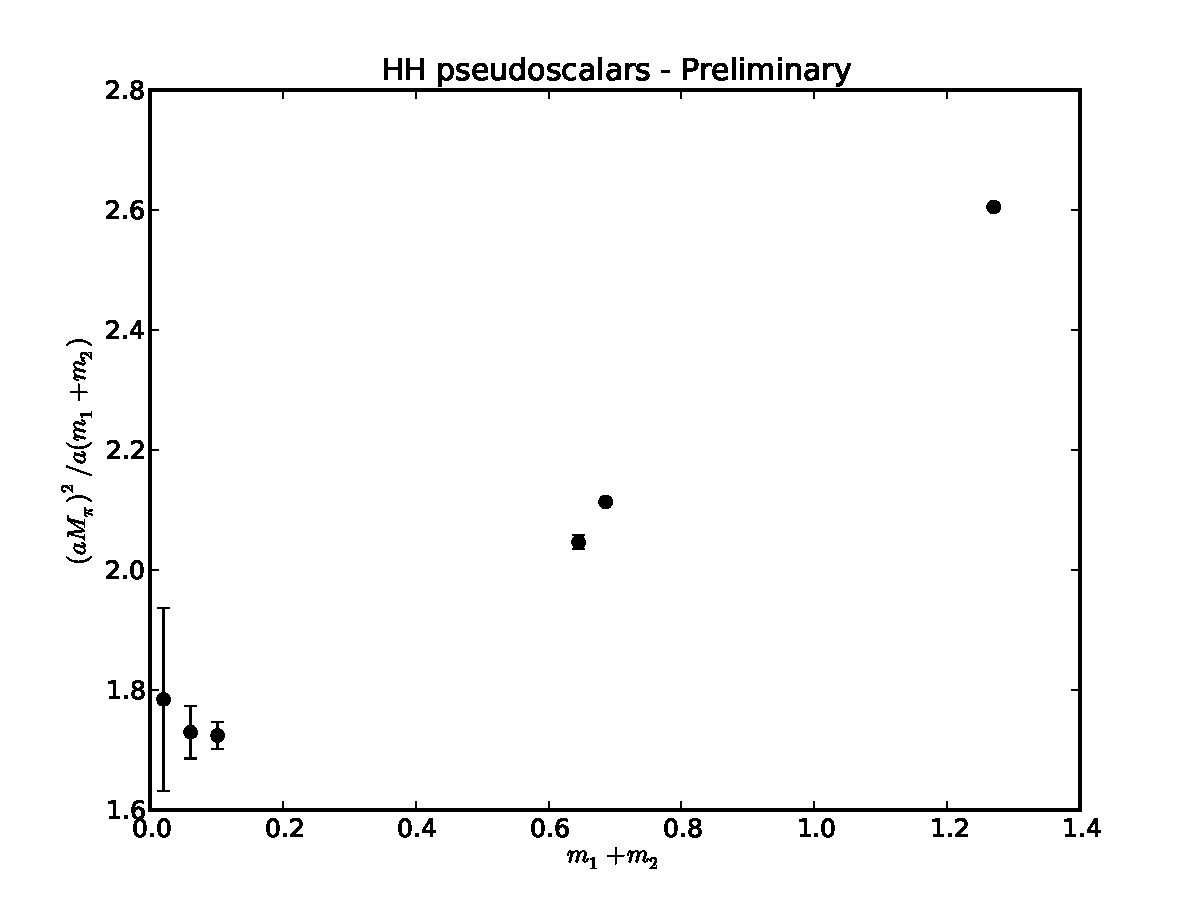
\includegraphics[width=.8\textwidth]{HH_pseudo}
\caption{HISQ valence on HISQ sea.  We see flat behavior in the pion-kaon mass range, whereas
when including the charm mass clearly~\ref{ss'} breaks down.}
\label{HH_pseudo}
\end{figure}

HISQ propagators are constructed using a ``corner wall" source.  This source is 1 at all sites
$\{ (\mathbf{x}, t) \, | \, \mathbf{x} \% 2 = \mathbf{0} \text{ and } t = t_0\}$.

%---- Mixed action propagators. ----
\subsection{Mixed action propagators.}
The \emph{Wilsonized} staggered propagator is given by the relation
\begin{equation}
D_{\psi_s}(x;y) = \Omega(x) \Omega^{\+}(y) D_{\chi}(x;y) \,,
\end{equation}
where $\Omega(x) = \prod_{\mu} (\gamma_\mu)^{x_\mu}$ is the Kawamoto-Smit transformation
and $D_{\chi}(x;y)$ is the naive staggered propagator.
All of the spin degrees of freedom are contained in the product of $\Omega$s.

In order to combine the Wilsonized propagator with the overlap propagator,
we need to ensure that both propagators share the same $\gamma$ conventions.
The overlap propagators are written (and read) using the Kentucky convention.
The only remnant of gamma matrices in the staggered propagator is via the staggered
phase conventions $\eta_\mu(x)$.  
These are equivalent to specifying precisely the Kawamoto-Smit transformation,
but do \emph{not} depend on the gamma convention used.  
Thus we need to ensure the correct ordering of the gammas in $\Omega(x)$,
 where the gamma matrix conventions are taken as Kentucky.
 There is an implementation of the conversion in MILC v7 {\tt staggered2naive.c}.
 For now I am assuming that the correct transformation follows that, 
 i.e.\ the HISQ phase conventions for the lattices I have follow that indicated here in the MILC code.
 
 
  \begin{figure}[h]
 \centering
 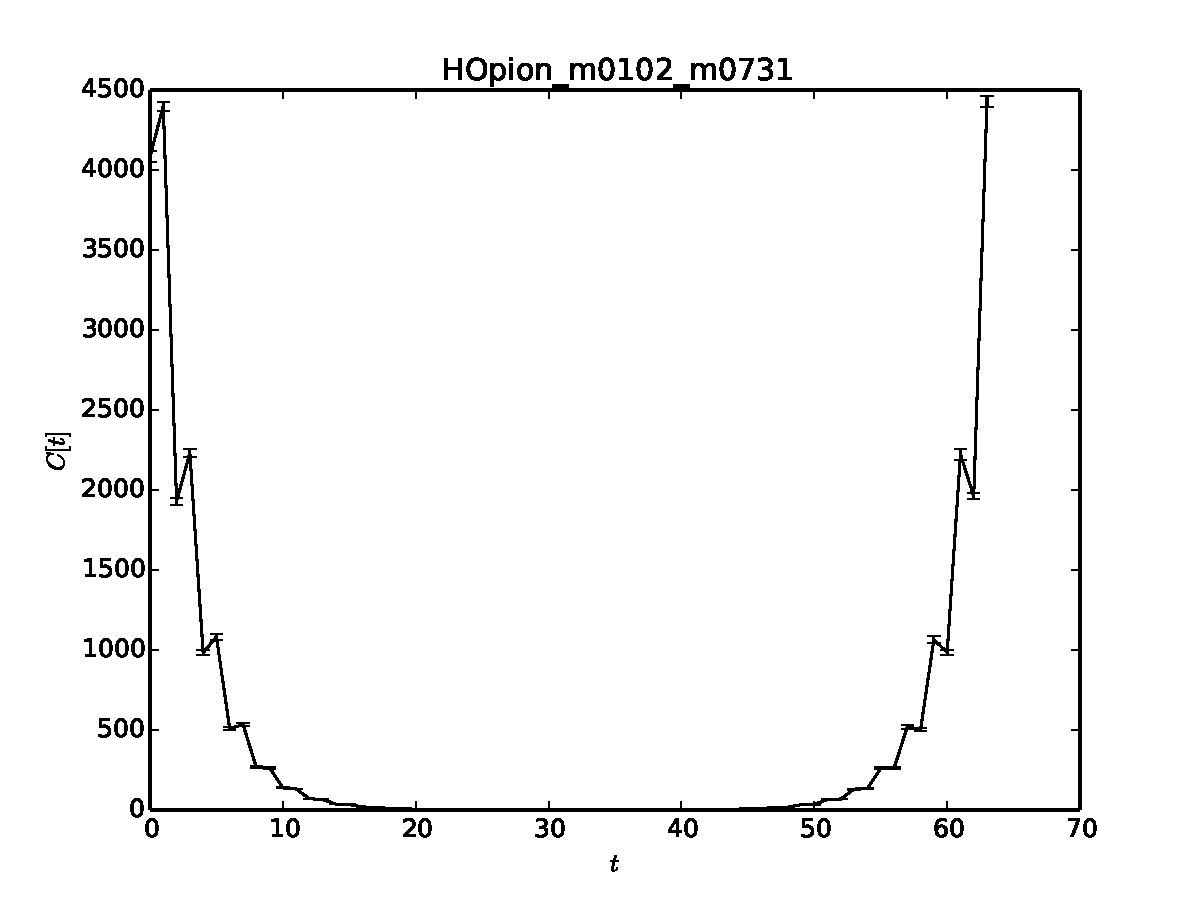
\includegraphics[width=.8\textwidth]{HOpion_m0102_m0731.pdf}
 \caption{}
 \end{figure}
 
 \begin{figure}[h]
 \centering
 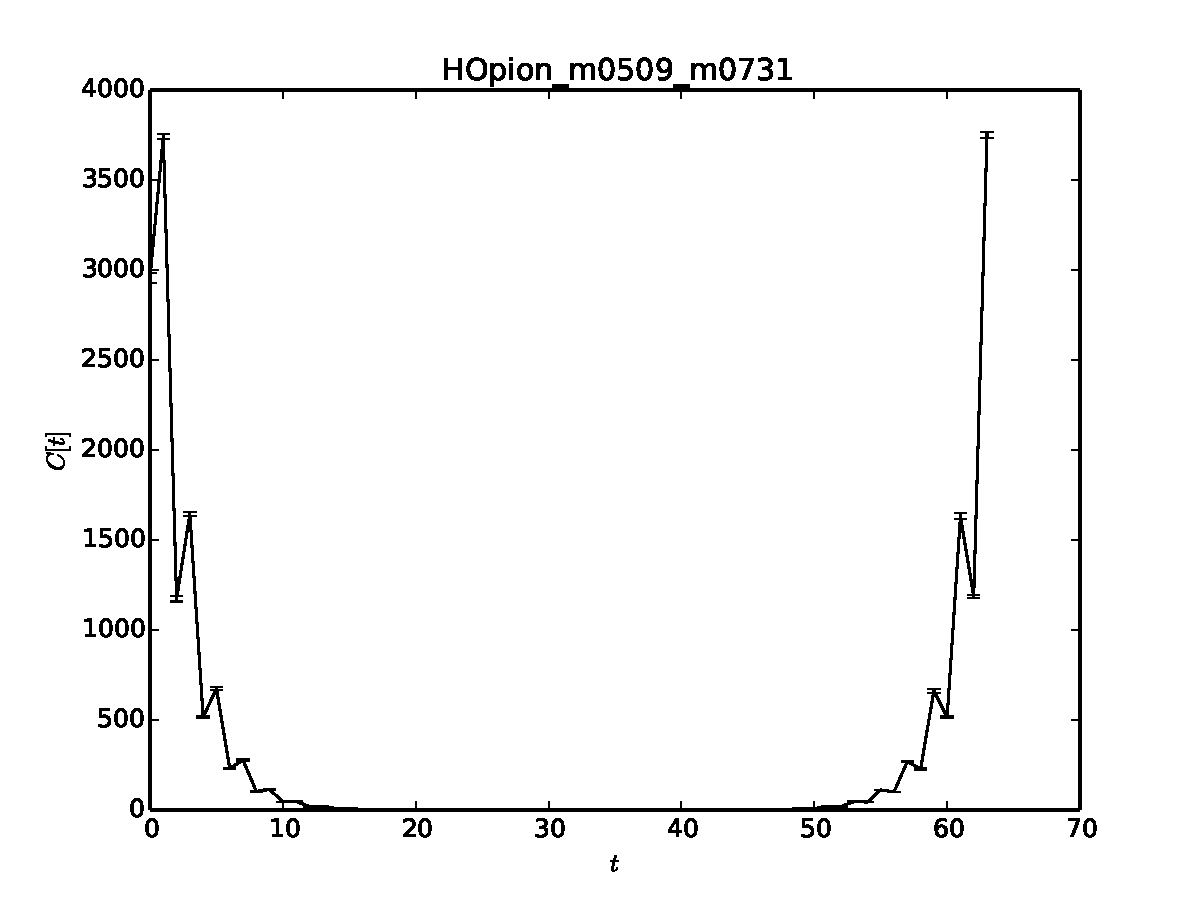
\includegraphics[width=.8\textwidth]{HOpion_m0509_m0731.pdf}
 \caption{}
 \end{figure}
 
  \begin{figure}[h]
 \centering
 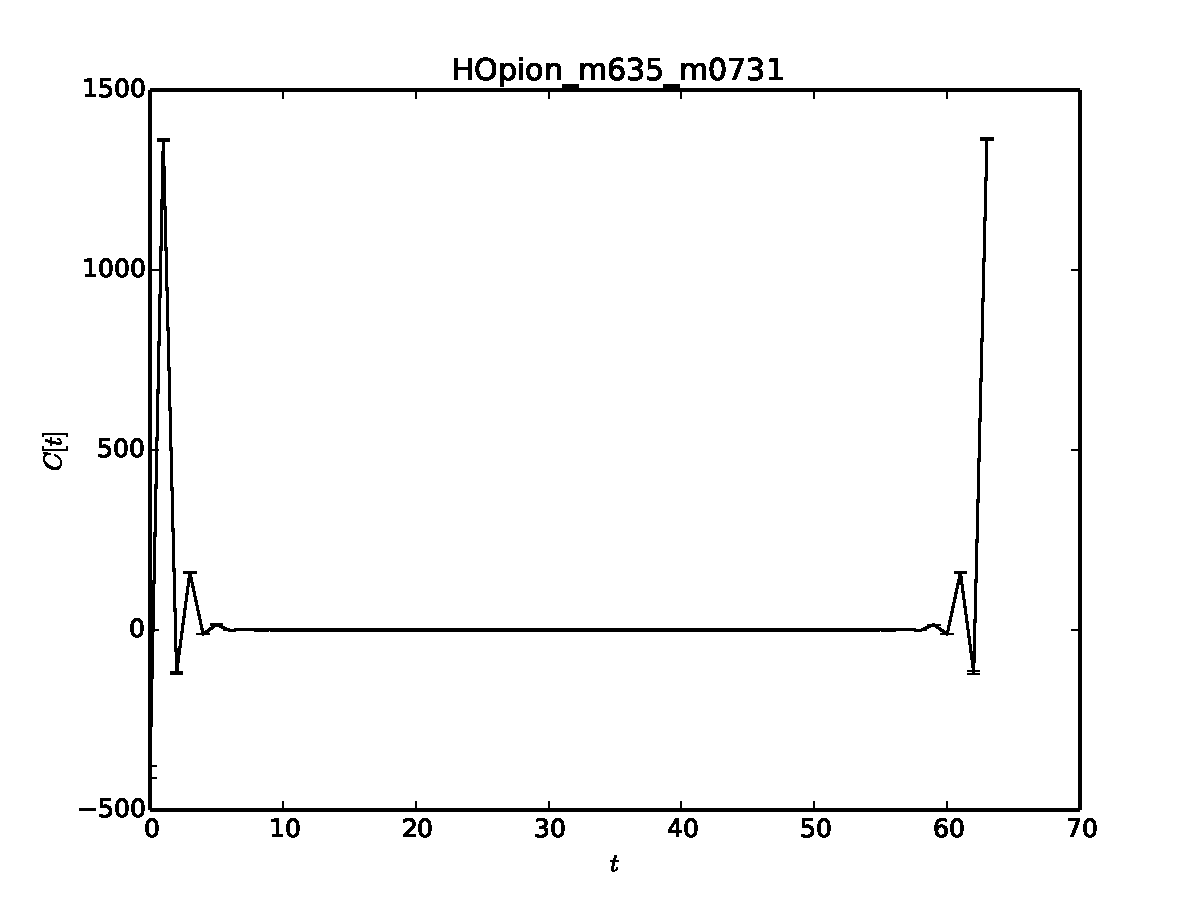
\includegraphics[width=.8\textwidth]{HOpion_m635_m0731.pdf}
 \caption{}
 \end{figure}
 
\begin{figure}[h]
 \centering
 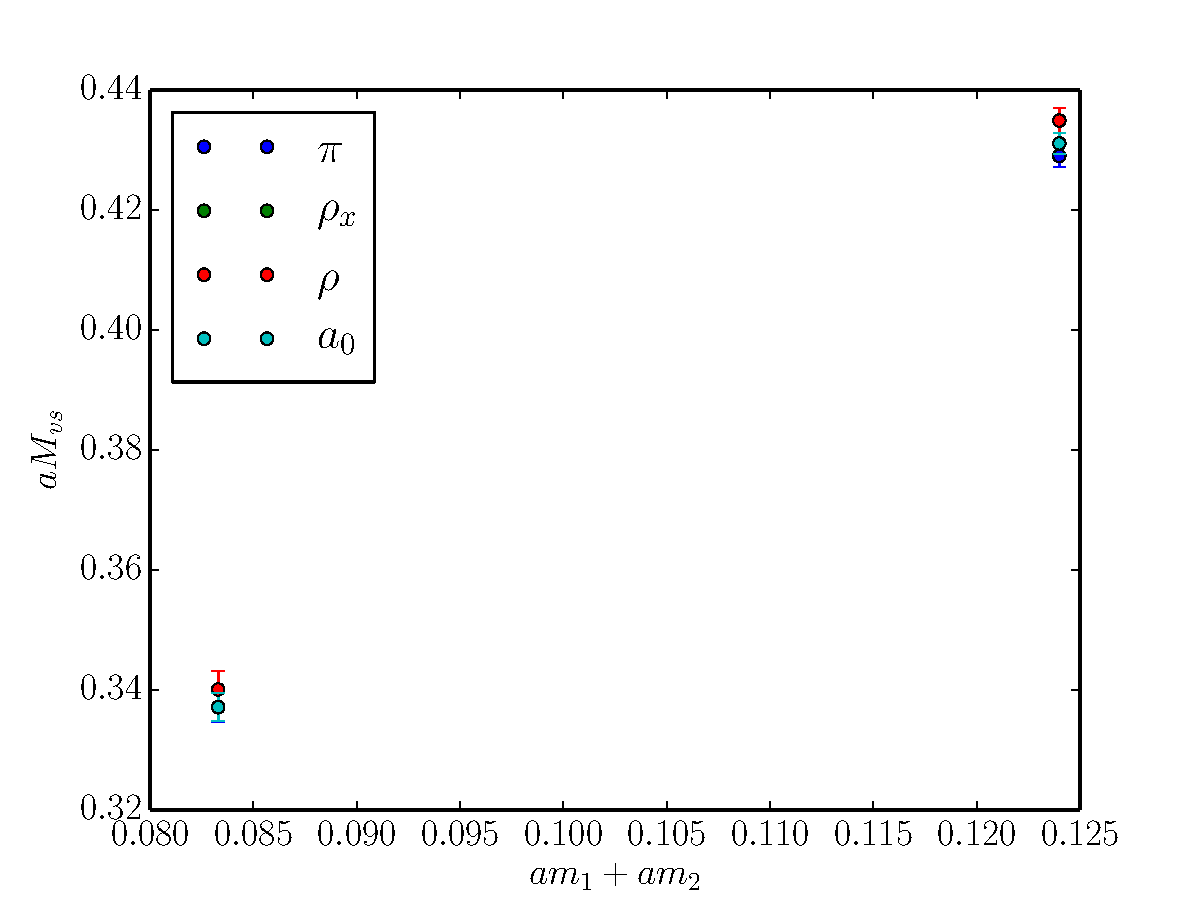
\includegraphics[width=.8\textwidth]{mixed_mpi.pdf}
 \caption{Preliminary plot of pion masses extracted from various mixed-action
 correlation functions.  Data involving charm is not included.}
\end{figure}

\begin{figure}[h]
 \centering
 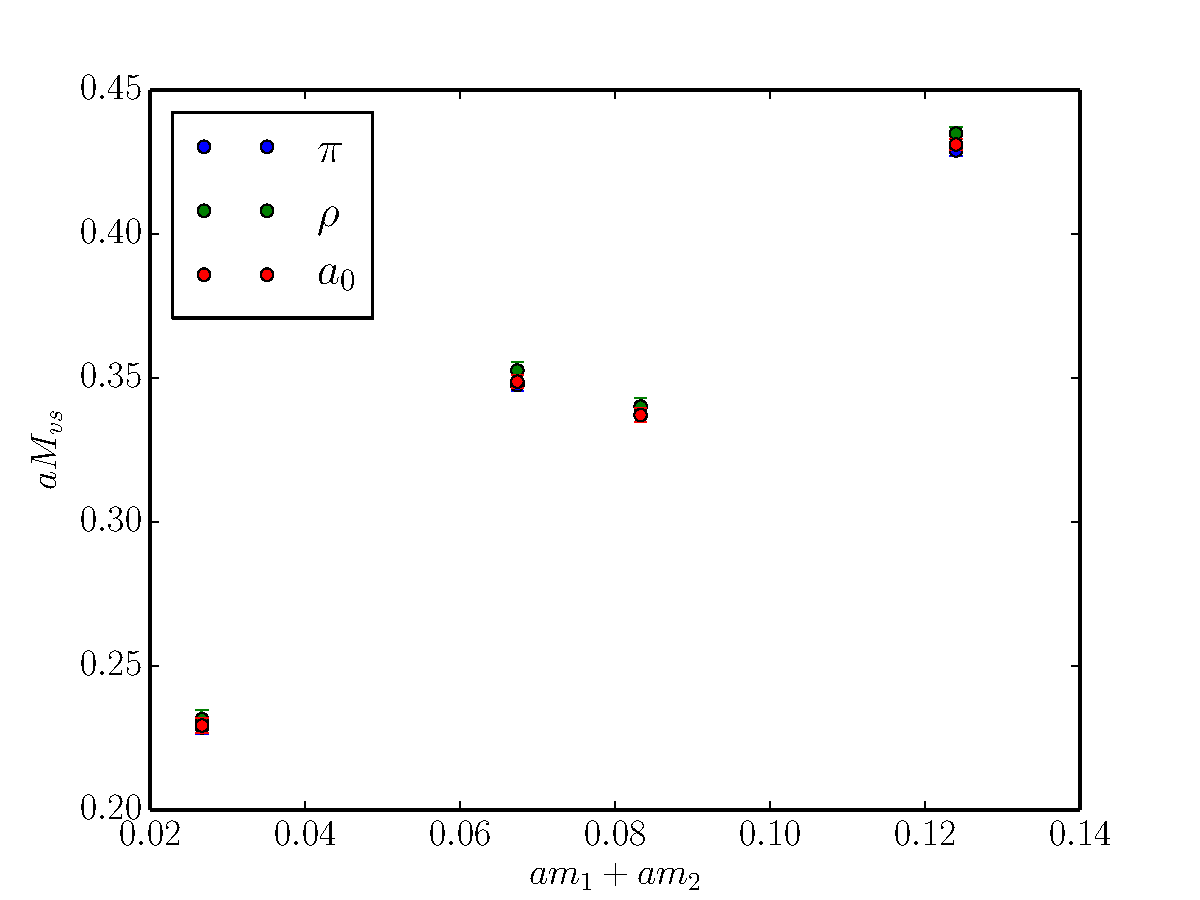
\includegraphics[width=.8\textwidth]{mixed_mpi2.pdf}
 \caption{Preliminary plot of pion masses extracted from various mixed-action
 correlation functions. 
 The masses are (HISQ, ov): (0102, 0165), (0509, 0165), (0102, 0731), (0509, 0731).
 For some reason $\rho_x$ data was very noisy for lightest
 two points and I threw it out.}
\end{figure}

\clearpage

%---- Measuring Delta_mix ----
\subsection{Measuring $\Dmix$.}
Combining Eqs.~\eqref{ss'} and~\eqref{vs} we have
\begin{equation}
\delta m^2 \equiv m^2_{vs} - m^2_{ss}/2 = B_{\text{ov}} m_v + a^2 \Dmix \, ,
\end{equation}
so that one can try to read off $a^2 \Dmix$ from the intercept of $\delta m^2(m_v)$. 
This is the measurement approach taken in~\cite{Lujan:2012wg}.
One could alternatively look at 
$\delta' m^2(m_s)  \equiv m^2_{vs} - m^2_{vv}/2$ (e.g.~\cite{Aubin:2008wk})
or the quantity $\Delta m^2 \equiv m^2_{vs} - m^2_{vv} - m^2_{ss}$ (e.g.~\cite{Orginos:2007tw}).
Presumably these approaches are equivalent.  
Figure~\ref{fig:delta_msq} shows a preliminary plot of $\delta m^2(m_v)$.
\begin{figure}
\centering
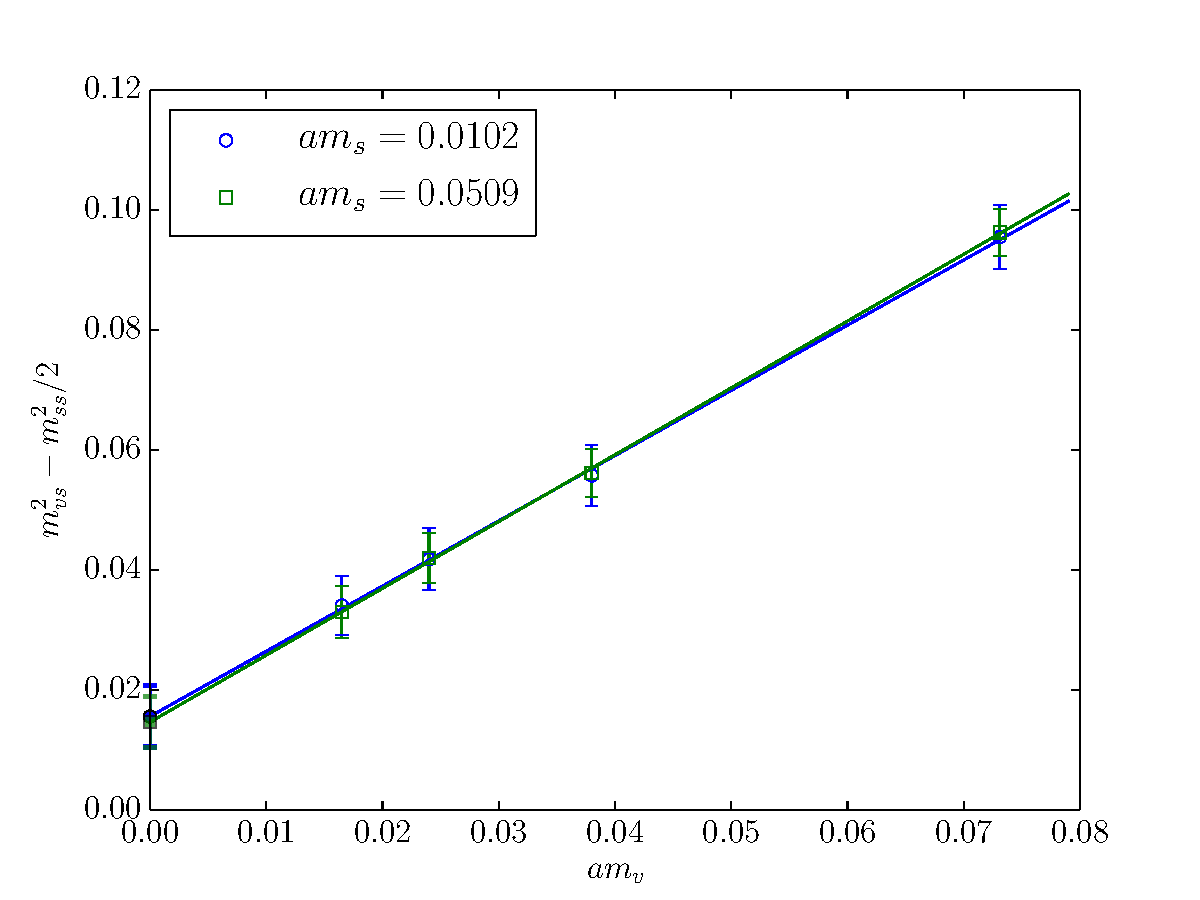
\includegraphics[width=\textwidth]{delta_msq.pdf}
\caption{(Very) preliminary determination of $a^2 \Dmix$ from the $24^3$ ensemble, using
two different values of the HISQ mass $m_s$. The data points are correlated, which
iss not taken account in the straight-line fit, and the pion masses themselves were determined
using uncorrelated fits.  Nevertheless the data is well-approximated by a straight line, is
insensitive to $m_s$, and has a small but non-zero intercept.} 
\label{fig:delta_msq}
\end{figure}

\begin{figure}
\centering
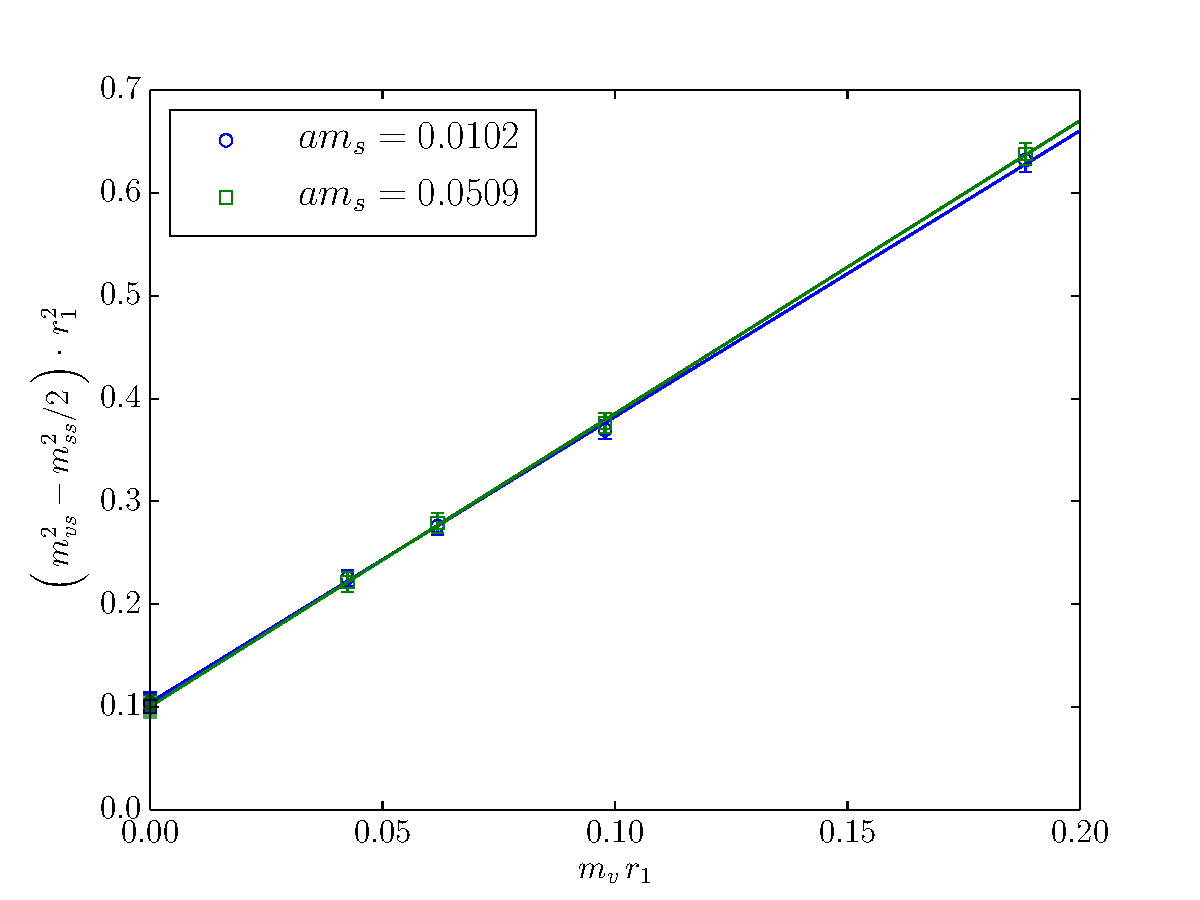
\includegraphics[width=\textwidth]{delta_msq_correlated.pdf}
\caption{Error bars calculated via correlated jackknife; results scaled by factors of $r_1/a$.}
\end{figure}

 
 \clearpage
%---- Appendix ----
\section{Appendix} 
Based on email with Nilmani (Apr 27, 2014) and prior emails with Padmanath.\\
See also notebook {\tt gamma\_conventions.nb}.\\
(anti)MILC conventions, used for inverting the overlap operator:
\begin{equation}
\begin{split}
\gamma_1 &= 
\begin{pmatrix}
 0 & 0 & 0 & -i \\
 0 & 0 & -i & 0 \\
 0 & i & 0 & 0 \\
 i & 0 & 0 & 0
\end{pmatrix}
\quad
\gamma_2 =
\begin{pmatrix}
 0 & 0 & 0 & 1 \\
 0 & 0 & -1 & 0 \\
 0 & -1 & 0 & 0 \\
 1 & 0 & 0 & 0
\end{pmatrix}
\\ \\
\gamma_3 &=
\begin{pmatrix}
 0 & 0 & -i & 0 \\
 0 & 0 & 0 & i \\
 i & 0 & 0 & 0 \\
 0 & -i & 0 & 0
\end{pmatrix}
\quad
\gamma_4 =
\begin{pmatrix}
 0 & 0 & -1 & 0 \\
 0 & 0 & 0 & -1 \\
 -1 & 0 & 0 & 0 \\
 0 & -1 & 0 & 0
\end{pmatrix}
\end{split}
\end{equation}
Kentucky conventions, used for writing the overlap propagator:\\
\begin{align}
\g_{1,\text{K}} &= \g_{1,\text{aM}} \\
\g_{2,\text{K}} &= - \g_{2,\text{aM}} \\
\g_{3,\text{K}} &= \g_{3,\text{aM}} 
\end{align}

\begin{equation}
\gamma_4 =
\begin{pmatrix}
 1 & 0 & 0 & 0 \\
 0 & 1 & 0 & 0 \\
 0 & 0 & -1 & 0 \\
 0 & 0 & 0 & -1
\end{pmatrix}
\end{equation}
Transformation matrix, implemented for example in {\tt io\_kentucky.c}:
\begin{equation}
T = \frac{1}{\sqrt{2}}
\begin{pmatrix}
 1 & 0 & 0 & 0 \\
 0 & 1 & 0 & 0 \\
 0 & 0 & -1 & 0 \\
 0 & 0 & 0 & -1
\end{pmatrix}
\end{equation}
 

%-------------------Bibliography-------------------

\bibliographystyle{JHEP}
\bibliography{\ROOT/myrefs}

\end{document}  